\documentclass[10pt, titlepage]{article} 

\usepackage[utf8x]{inputenc}
\usepackage{fullpage}
\usepackage{graphicx}
\usepackage{amsfonts}
\usepackage{amsmath}

\title{Applications of Cryptographically Enforced Access Control \\ Interim Report}
\author{Daniel Randall}
\date{}

\begin{document}
\maketitle

\begin{abstract}
Abstract
\end{abstract}

\renewcommand{\abstractname}{Acknowledgements}
\begin{abstract}
Acknowledgements
\end{abstract}


% Create the contents page
\newpage
\tableofcontents
\newpage

\newcommand{\defeq}{\stackrel{\textup{\tiny def}}{=}}

\section{Introduction}
The problem taken on by this product is that of implementing a concrete application of modern cryptographically enforced access control techniques. This problems stems from changes in the last decade, mainly due to the huge popularity of the internet, which has seen a big increase in the amount of open information available and methods those with malicious intent can use to gain access to information which is protected. This has brought with it a focus from academics and corporations on controlling who has access to what information and how efficient and secure these techniques are. While a lot of recent research has been done on techniques to achieve this there are little freely available implementations of these techniques in a practical environment.
\newline \indent By building a Dropbox app this project aims to implement and analyse a selection of techniques for cryptographically enforced access control. To achieve this a structure will be developed, with care taken not to rely on any features to be tested and instead allow for easy plug-and-play for each feature such that all combinations can be easily analysed. The objectives are to find the extent of the strengths and weaknesses of the chosen proposals and those which work well together and those which are not able to work so well together. With these results the hope is that further insights will be generated as to where future work is needed. Another interesting result will be how well such cryptographically enforced access control measures are able to be used in a `everyday' environment such as the type which Dropbox offers.

\section{Background Research}
\subsection{Overview}
While protecting sensitive data from adversaries has been a concern for hundreds of years it was not until the First World War that the field of cryptography received serious academic attention however from then on the majority of the work was carried out secretively by states.\cite{appliedCryptoBook} Cryptography was only employed by the military until the 1970s where cheaper hardware reduced ``the design limitations of mechanical computing and brought the cost of high grade cryptographic devices down to where they can be used in such commercial applications as remote cash dispensers and computer terminals.\cite{newCryptoDirections}" And new methods of sharing keys such that they could be transferred over insecure channels and thus eliminate the need for physical contact (ie. couriers) before secure communication became possible. One such technique was a \textit{public key cryptosystem}, in which two distinct asymmetric keys are used. One for encrypting, which is made publically available, and one for decrypting, which is kept private, thus anyone can encrypt messages with the public key but only the owner of the private key may decrypt the messages. Also, more importantly to this project, the 1970s also saw the development of major publically known symmetric key ciphers such as Data Encryption Standard (DES). Since then improvements on such algorithms have been designed and cryptography has become an integral part of many businesses who use it, not only for privacy but, for many different reasons, such as: ``authentication (bank cards, wireless telephone, e-commerce, pay-TV), access control (car lock systems, ski lifts), payment (prepaid telephone, e-cash)."\cite{classicalCryptoBook}
\newline \indent Block ciphers (such as DES) are a type of symmetric key algorithms used to encrypt data. They map $n$-bit plain-text blocks to $n$-bit cipher-text blocks where $n$ is the length of the block. This mapping is one-to-one and thus invertible. The encryption function takes ``a $k$-bit key $K$, taking values from a subset $K$ (the key space) of the set of all $k$-bit vectors $V_{k}$." \cite{blockCiphers} Block ciphers are deterministic and so with the same key and the same plain-text, one should receive the same cipher-text.
\newline \indent This project focuses on access control as the application of cryptography. The purpose of access control is to ``limit the actions or operations that a legitimate user of a computer system can perform. Access control constrains what a user can do directly, as well as what programs executing on behalf of the users are allowed to do."\cite{accessControlPrinciples} For instance, many operating systems control access to files by assigning permissions to users (eg. read, write, execute.) Typically vanilla access control is based on capabilities or access control lists (ACLs). ACLs works by assigning each object its own ACL detailing for each user which permissions she is authorised to perform on the object. With this setup it is easy to add, edit or remove user permissions and it is easy to see what users have permissions for each object, however all ACLs need to be accessed to determine what objects a user currently has access to. Capabilities are similar to ACLs however each user is associated with a list instead of an object and all capability lists need to examined to determine which users can access a particular object. An example of this, similar to what would be deployed in an OS, can be viewed in Figure ~\ref{fig:capabilities} where 'R' refers to read, 'W' to write and 'Own' signifies that that user is the owner of the object.
\newline
\newline This project is an implementation of the latest theories and ideas on how to securely and efficiently create a solution for hierarchical a for access control. The concrete application domain chosen has been chosen as a public Dropbox. The reasons for this are that the folder structure implemented by filesystems, and incorporated by Dropbox, naturally conform to the strict hierarchy requirements by the chosen encryption method. Dropbox is incredibly popular, with over 100 million users collectively saving 1 billions files per day.\cite{dropboxInfo}
\newline \indent An appropriate alternative application could have been a content distribution network such as BitTorrent\cite{bittorrent}, however due to a number of different clients being used (Utorrent, Deluge...), many different ways to connect to the tracker (.torrent files, magnetic links...) as well as inconsistent performance when using BitTorrent meant that testing the implementation would have posed a much more difficult task.

\begin{figure}
\centerline{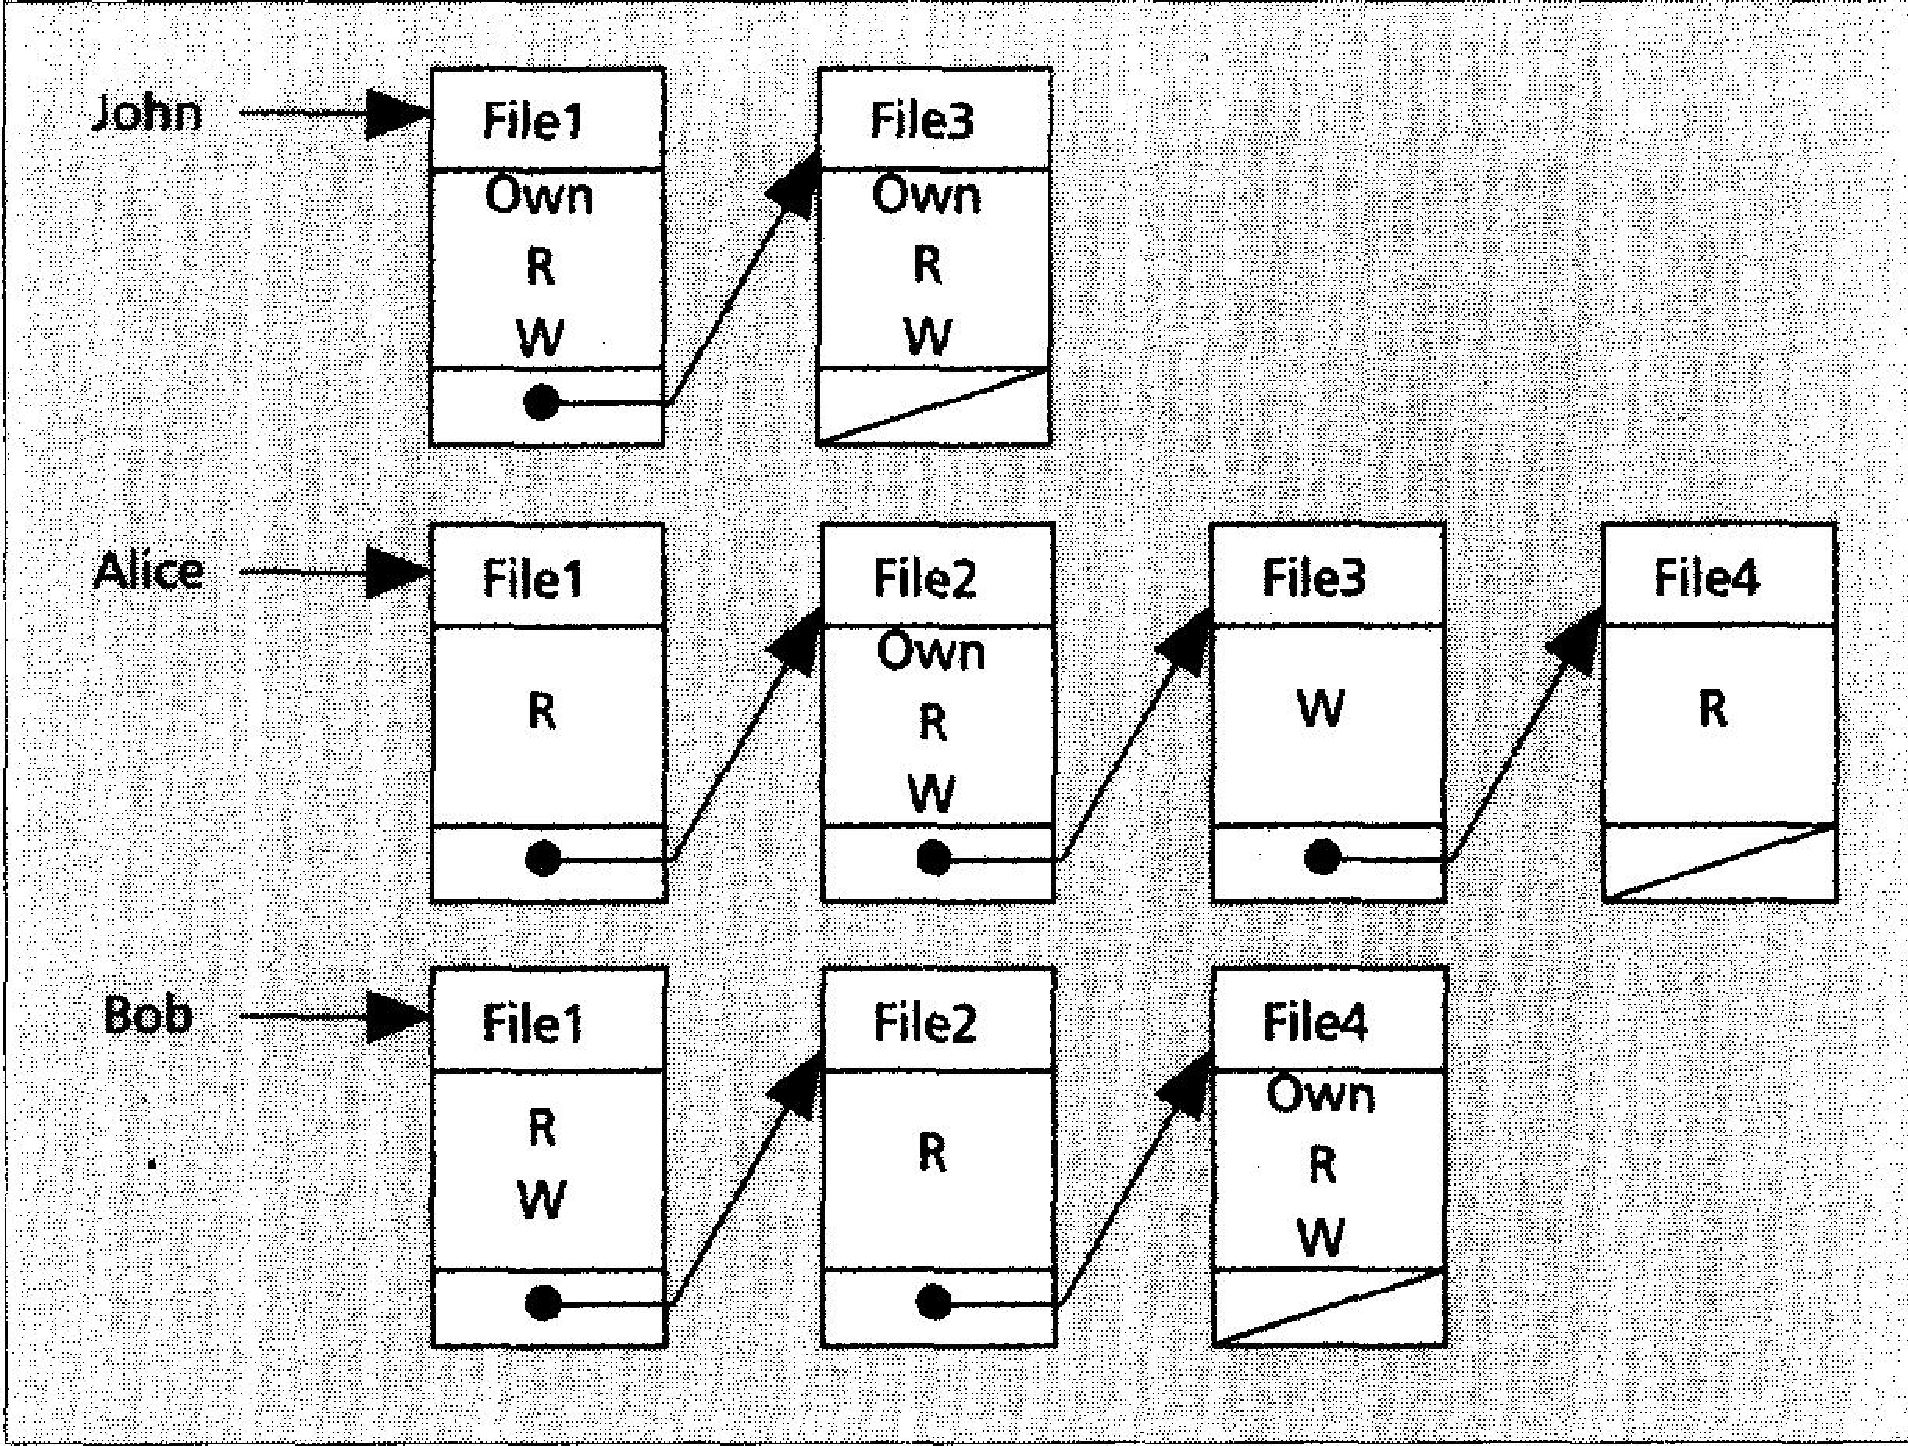
\includegraphics[height=2.5in,width=4in,angle=0]{capabilities.pdf}}
\caption{Capabiliy list for four files and three users.\cite{accessControlPrinciples}}
\label{fig:capabilities}
\end{figure}

\subsection{Technical Research}

\subsubsection{Hierarchical Cryptography for Access Control}
Hierarchical access control relies on different levels (or classes) of security which can be represented as labels in a partially ordered set (L, $≤$). These labels can be applied to users, $u$, and objects, $o$, using a many-to-many labelling function $lambda : U ∪ O → L$ where $U$ is a set of all users $u$ and $O$ is a set of all objects $o$. "$u$ is authorized to access $o$ if and only if $\lambda(u)≤\lambda(o)$\cite{mainPaper}."

\subsubsection{Interval-Based Access Control}
Interval-based access control works in a similar way to standard hierarchical access control however, unlike standard hierarchical access control, it is necessary to have a lower bound of access as well an upper bound. If $1, \dots , n$ is a totally ordered set of all possible security levels and $[x,y]$, where $1≤x≤y≤n$, is an interval associated with some user then that user can access an object $o$ associated with a security level $l$ where $1≤l≤n$ if and only if $l ∈ [x,y]$.
\newline \indent This idea can be extended to cover $k$-dimensional cardinalities:
\newline \indent ``Let $O$ be a set of protected objects, let $U$ be a set of users, and let $A_{1}, \dots , A_{k}$ be finite, totally ordered sets of cardinality $n_{1} , \dots , n_{k}$, respectively. We write $\mathcal{A}$ to denote $\prod_{i=1}^k A_{i} = A_{1} \times \dots \times A_{k}$.  
\newline \indent We say $[x_{i},y_{i}] ⊆ A_{i}$, where $1≤x_{i}≤y_{i}≤n_{i}$, is an \textit{interval} in $A_{i}$. We say that $\prod_{i=1}^k [x_{i},y_{i}] = [x_{1},y_{1}] \times \dots \times [x_{k},y_{k}] ⊆ \mathcal{A}$ is a \textit{hyperrectangle}. We write HRec($\mathcal{A}$) to denote the set of hyperrectangles in $\mathcal{A}$.
\newline \indent We assume that each object $o ∈ O$ is associated with a unique attribute tuple $(a_{1} , \dots , a_{k}) ∈ A$, and each user $u ∈ U$ is authorized for some hyperrectangle $\prod_{i=1}^k [x_{i},y_{i}] ∈$ HRec($\mathcal{A}$). Then we say that a user $u$ associated with $\prod_{i=1}^k [x_{i},y_{i}]$ is \textit{authorized} to read an object $o$ associated with tuple $(a1 , . . . , ak) ∈ \mathcal{A}$ if and only if $a_{i} ∈ [x_{i},y_{i}]$ for all $i$\cite{mainPaper}."
\newline \indent Some common implementations of this scheme are\cite{mainPaper}:
 \begin{itemize}
 \item \textit{Temporal} ($k=1$) where $\mathcal{A} = A_{1}$ and each integer in $1, \dots , n ∈ \mathcal{A}$ are in one-to-one correspondence with the time points. A 1-dimensional scheme follows the regular interval-based access control scheme as described above in which a user is associated with an interval $[x,y]$ and each object is associated with an integer. If the integer exists in the interval then the user should possess, or have the means to possess, the key to access the object.
 \newline \indent An example of this can be seen in Figure ~\ref{fig:hasse}. For instance if a user was associated with the interval [2,4] then she should be be able to derive the keys for the leaf nodes [2,2], [3,3] and [4,4] but should not be able to derive the key to access the leaf node [1,1].
 \item \textit{Geo-spatial} ($k=2$) where $\mathcal{A} = A_{1} \times A_{2}$. $\mathcal{A}$ represents a finite rectangular $m \times n$ grid of cells for which objects and keys are associated with a unique cell. Users are associated with an interval which correspond to a subrectangle of $\mathcal{A}$ where the user is able to derive keys for all cells in the area\cite{atallahGeo}.  More formally, ``each object is associated with
some point (x, y) and each user is associated with some rectangle $[x_{1} , y_{1} ] \times [x_{2} , y_{2} ] = (t_{1} , t_{2} ) : t_{1} ∈ [x_{1} , y_{1} ], t_{2} ∈ [x_{2} , y_{2} ]$.
We write $T_{m,n}$ (as an abbreviation of the more accurate $T_{m} \times T_{n}$) to denote the set of rectangles defined by a rectangular $m \times n$ grid of points: that is, $T_{m,n} \defeq [x_{1} , y_{1} ] \times [x_{2} , y_{2} ] : 1 ≤ x_{1} ≤ y_{1} ≤ m, 1≤x_{2}≤y_{2}≤n$"\cite{mainPaper}. Leaf nodes make up the $m \times n$ grid and are of the form $[x, x] \times [y, y]$ or $[x, y]$.
\newline \indent Two visualisations of this can be seen in Figure ~\ref{fig:geospatial}. Figure ~\ref{fig:geospatial}a displays $T_{2,2}$ as a "partially ordered set of subsets ordered by subset inclusion in which rectangles are represented by filled circles," while the second depicts $T_{2,2}$ where "nodes of the same color have the same area
(as rectangles): all rectangles of area 2 are filled in gray, whereas all rectangles of area 1 are filled white."\cite{mainPaper}
 \end{itemize}
 
\begin{figure}
\centerline{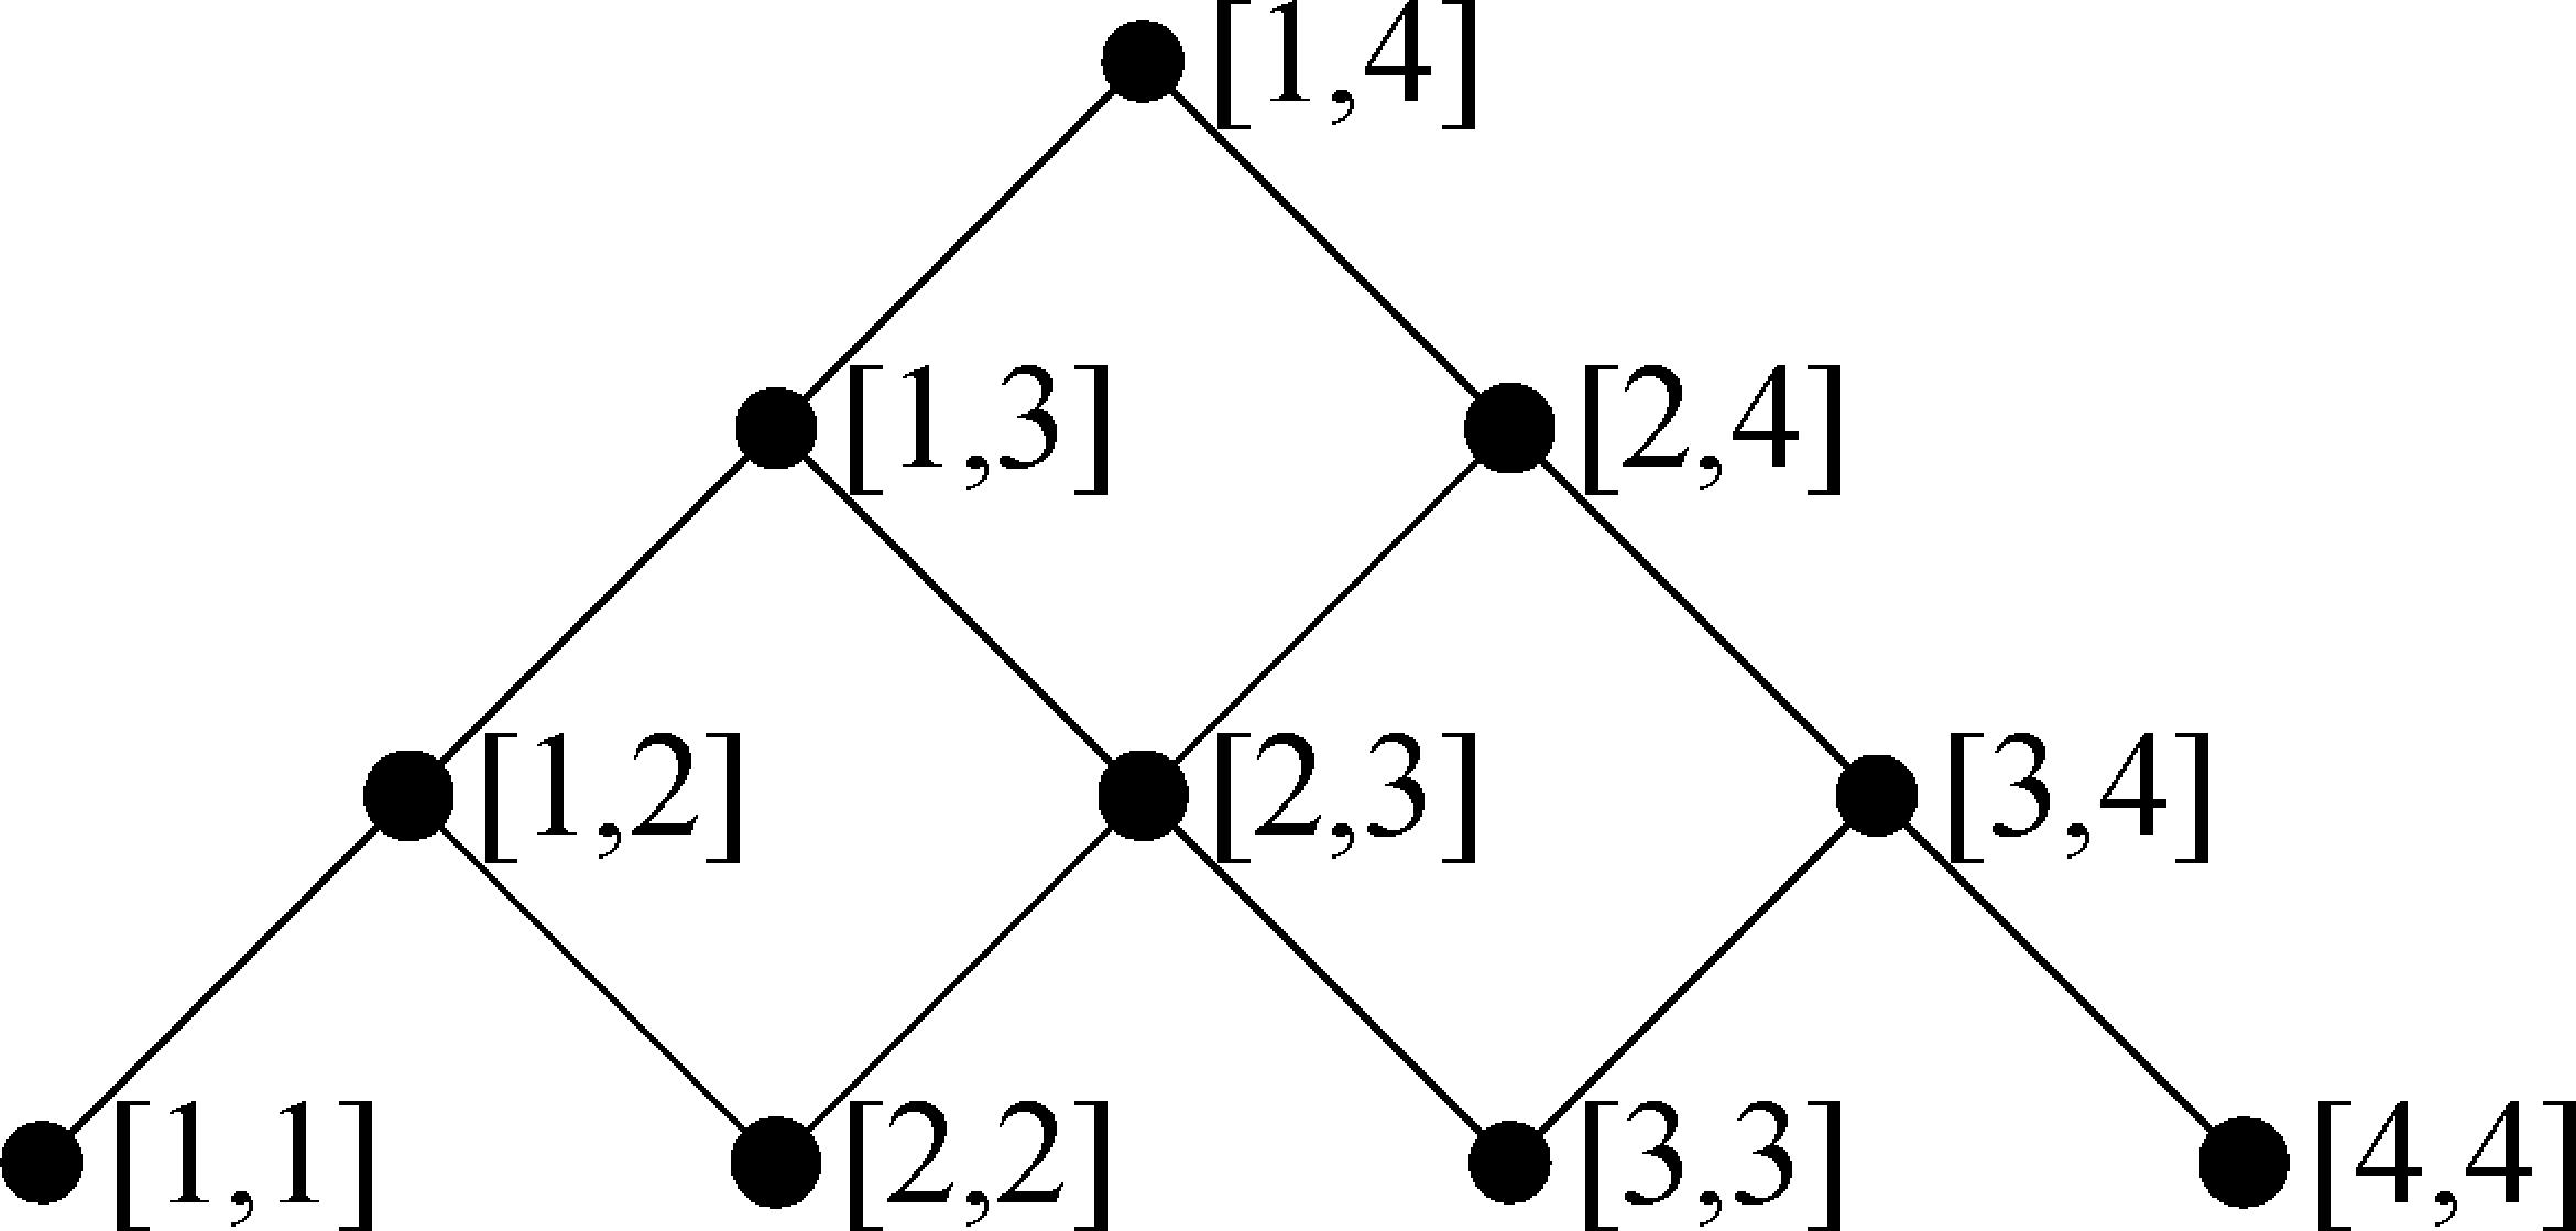
\includegraphics[height=1.0in,width=2in,angle=0]{hasse.pdf}}
\caption{The Hasse diagram of (T4 , $⊆$).\cite{mainPaper}}
\label{fig:hasse}
\end{figure}

\subsubsection{Key Assignment Schemes (KAS)}
A key assignment scheme (KAS) controls the information flow through the tree. The scheme dictates how a user is to derive access to objects she is permitted access to as well as preventing her access to objects she is forbidden from viewing. KAS are ``usually evaluated by the number of total keys the system must maintain, the number of keys each user receives, the size of public information, the time required to derive keys for access classes, and the work needed when the hierarchy or the set of users change.\cite{atallah2005}" As an example, the simplest possible KAS would be to assign every single key for which $k(y) : y<\le(u)$ where $u$ is a user and $le$ is a labelling function. This scheme, however, is not ideal and efforts are generally make to reduce the number of keys held by the user. To do this most schemes look to either provide additional public or private information. 
\newline \indent Recently a lot of work has been done in key assignment schemes, however not all of the proposed solutions are secure or efficient. As observed by Blanton[2007], the most efficient of the solutions achieve the following properties\cite{blanton2007}:
\begin{itemize}
\item Each node in the access graph has a single secret key associated with it.
\item The amount of public information for the key assignment scheme is asymptotically the same as that needed to represent the graph itself.
\item Key derivation involves only the usage of efficient cryptographic primitives such
as one-way hash functions.
\item Given a key for node $v$, the key derivation for its descendant node $w$ takes \textit{l} steps, where \textit{l} is the length of the path between $v$ and $w$.
\end{itemize}
 A few potential algorithms to test will be outlined here:
\begin{itemize}
\item \textbf{Iterative key encrypting (IKE)} - For each edge in the graph the child key is encrypted with the parent key and published as public information. The user is then, using a single private key, able to iteratively derive any child key using that information\cite{lazyEncryption}. The AFB scheme by Atallah et al. is an example of this KAS, offering\cite{atallah2005}:
\begin{itemize}
\item A single private key held by the user
\item Permits only a hash functions to derive keys
\item Derivation of a descendant node's key requires $\mathcal{O}(l)$ operations where $l$ is the length of the path between the nodes
\item "Updates [i.e., revocations and additions] are handled locally and do not propagate to descendants or ancestors of the affected part of G"
\item "The space complexity of the public information is the same as that of
storing [the] graph."
\item Provably secure against collusion
\end{itemize}


\item \textbf{The Akl-Taylor scheme} - Created by Akl and Taylor, this node-based scheme is the first KAS created. Key derivation in a node-based scheme eliminates the need for recursive calculations, instead the algorithm works as follows\cite{lazyEncryption}:
\begin{itemize}
\item The RSA key generator is called to obtain $(n, e, d)$, of which only n is used
\item $s$ is chosen at random from $\mathbb{Z}^{*}_{n}$
\item A mapping is chosen $\phi \rightarrow \mathbb{N}^{*}$ such that $\phi(x) | \phi(y)$ if and only if $y≤x$.
\item The key for $x$, $k(x)$, is defined to be $k(x) = s^{ \phi (x)} \bmod n$.
\item ${n} \cup (\phi(x) : x ∈ L)$ is published publically.
\end{itemize}
where ``$(n, e, d)$ such that: $n = pq$, where $p$ and $q$ are distinct odd primes; $e ∈ \mathbb{Z}^{*}_{\phi(n)}$, where $\phi(n) = (p − 1)(q − 1)$, $e > 1$, and $(e, \phi(n)) = 1$; $d ∈ \mathbb{Z}^{*}_{\phi(n)}$, where $ed \equiv 1 \bmod \phi(n)$."
\newline Using private key $k(x)$ to derive $k(y)$ where $y≤x$ the following formula is used:
\begin{align*}
(k(x))^{\frac{\phi(y)}{\phi(x)}} = (s^{\phi(x)})^{\frac{\phi(y)}{\phi(x)}} = s^{\phi(y)} = k(y).
\end{align*}
where $\phi(x)$ and $\phi(y)$ is publically available information.
\newline \indent This scheme while secure (when $\phi$ is chosen appropriately) and fast, requires a lot of public information.
\end{itemize}
Some KASs for special case scenarios exist, such as for when the number of leaf classes is substantially larger than the number of non-leaf classes.\cite{largeLeaf} There has also recently been a number of works on elliptic curve cryptography (ECC)\cite{ecc1}\cite{ecc2}, however this method relies on public-key cryptography and this project will initially focus on symmetric key techniques.

\begin{figure}
\centerline{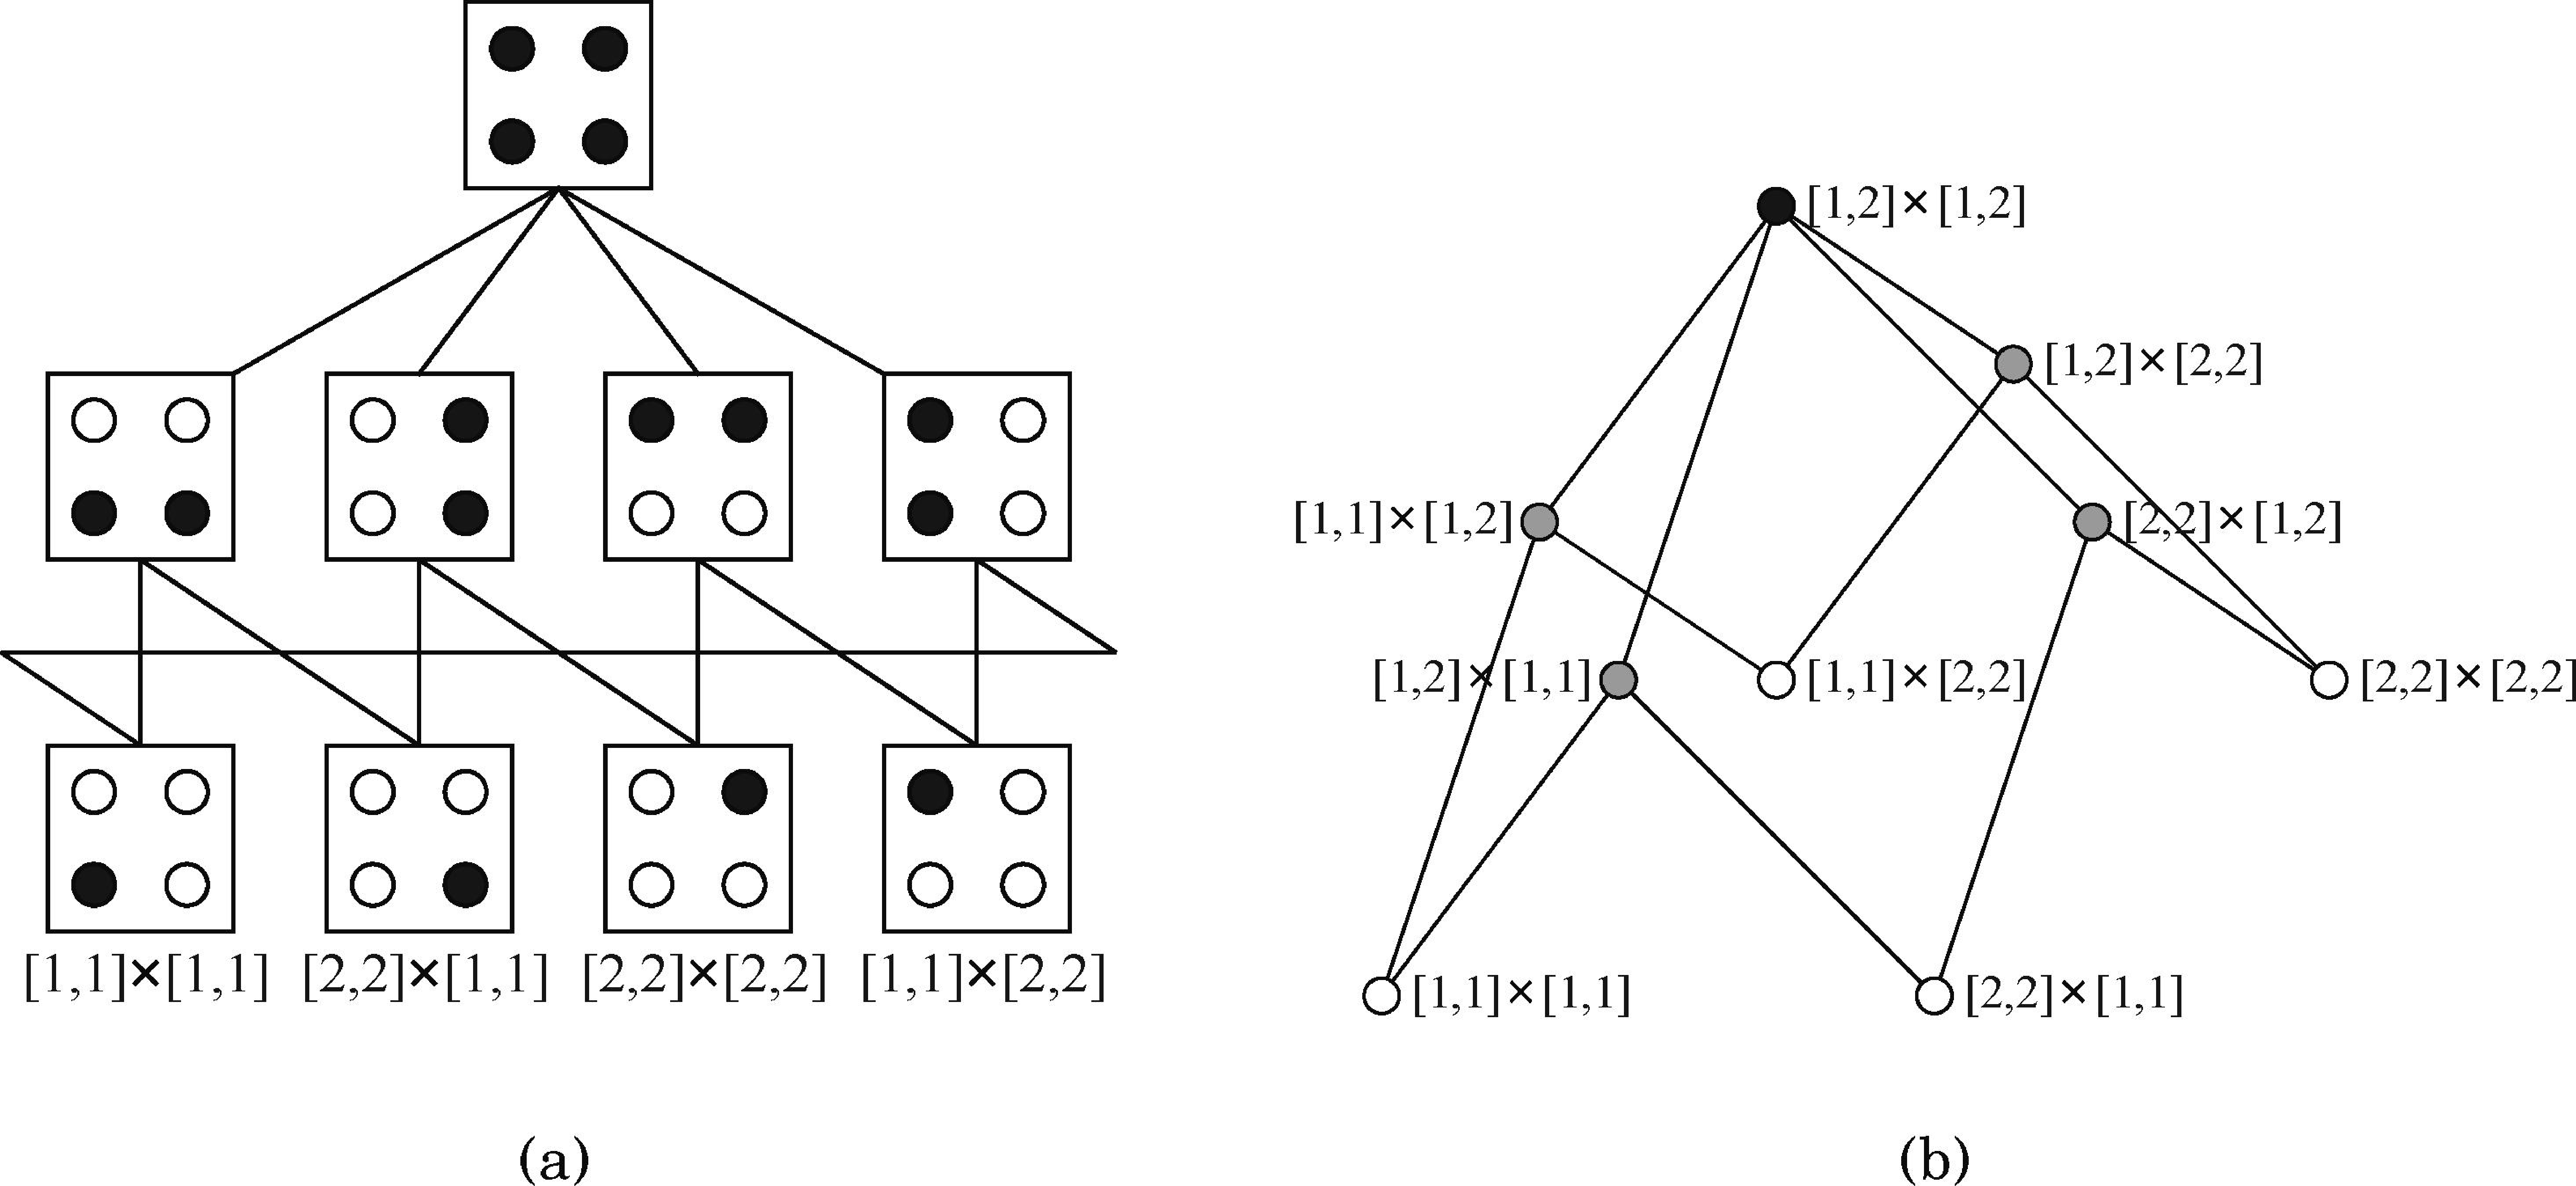
\includegraphics[height=3.0in,width=6in,angle=0]{geospatial.pdf}}
\caption{Two representations of $T_{2} \times T_{2}$.\cite{mainPaper}}
\label{fig:geospatial}
\end{figure}

\subsubsection{Revokation of Permissions and Re-encryption}
There are occasions where a user previously granted access at some security interval is later revoked of those permissions. If the user was associated with a security label $l$ then the revoked user has held a key which grants her access to objects at every node within her security interval, $l' \le l$. Due to this it is no longer acceptable to continue using the same key for any $l'$ as the revoked user would be able to view or edit future and existing objects that she should no longer have access to. Thus for every $l'$ it is necessary to replace the key associated with the label with a new key with which every object associated with $l'$ is re-encrypted with.
\newline \indent The most obvious way to achieve re-encryption is to immediately re-encrypt every object associated with every $l'$ the moment the user has been revoked and distribute the new keys to the appropriate users to replace the old key. This method ensures the revoked user has no access the objects she previously had access to, therefore providing robust security, and the users who have not had their permissions revoked continue as normal with the new key. However the number of objects associated with $l'$ may well be extremely large meaning that re-encrypting all of them instantly could take a long time, possibly disrupting the service. It also may well be the case that a significant number of the objects may not be viewed or edited for some time, if ever. An alternative to this method is \textit{lazy re-encryption}.
\newline \indent Lazy re-encryption does not instantly re-encrypt all objects, instead an object is re-encrypted with the newly assigned key for the security label $l'$ only when it is edited for the first time after the revokation by any user. The result is that the workload of re-encryption is spread out over time and is only performed when absolutely necessary. Employing lazy re-encryption requires the user to possess more than one key - one key for objects yet to be encrypted and one for objects encrypted with the new key.\cite{lazyEncryption} This means that the revoked user has the capacity to view objects while they remain unchanged and not yet re-encrypted. While logic suggests that the user who has been revoked has already been able to see the object during the time their permissions were valid meaning that it is unlikely to pose a real threat, this may not be acceptable in every scenario. To avoid this problem another solution may be to, instead of waiting for the object to be edited, wait for the object to be requested for a read. This way the user will need to possess the newly assigned key to read the object however the burden of re-encryption is still spread out over time. It can also be noted that if there are a number of users revoked over time and there are sporadic reads/writes of different files there will be a large number of keys being used for files associated with the same security level that a single user is required to hold. To keep the number of keys down it may be desirable at times to re-encrypt objects even when they are yet to be accessed.

\begin{figure}
\centerline{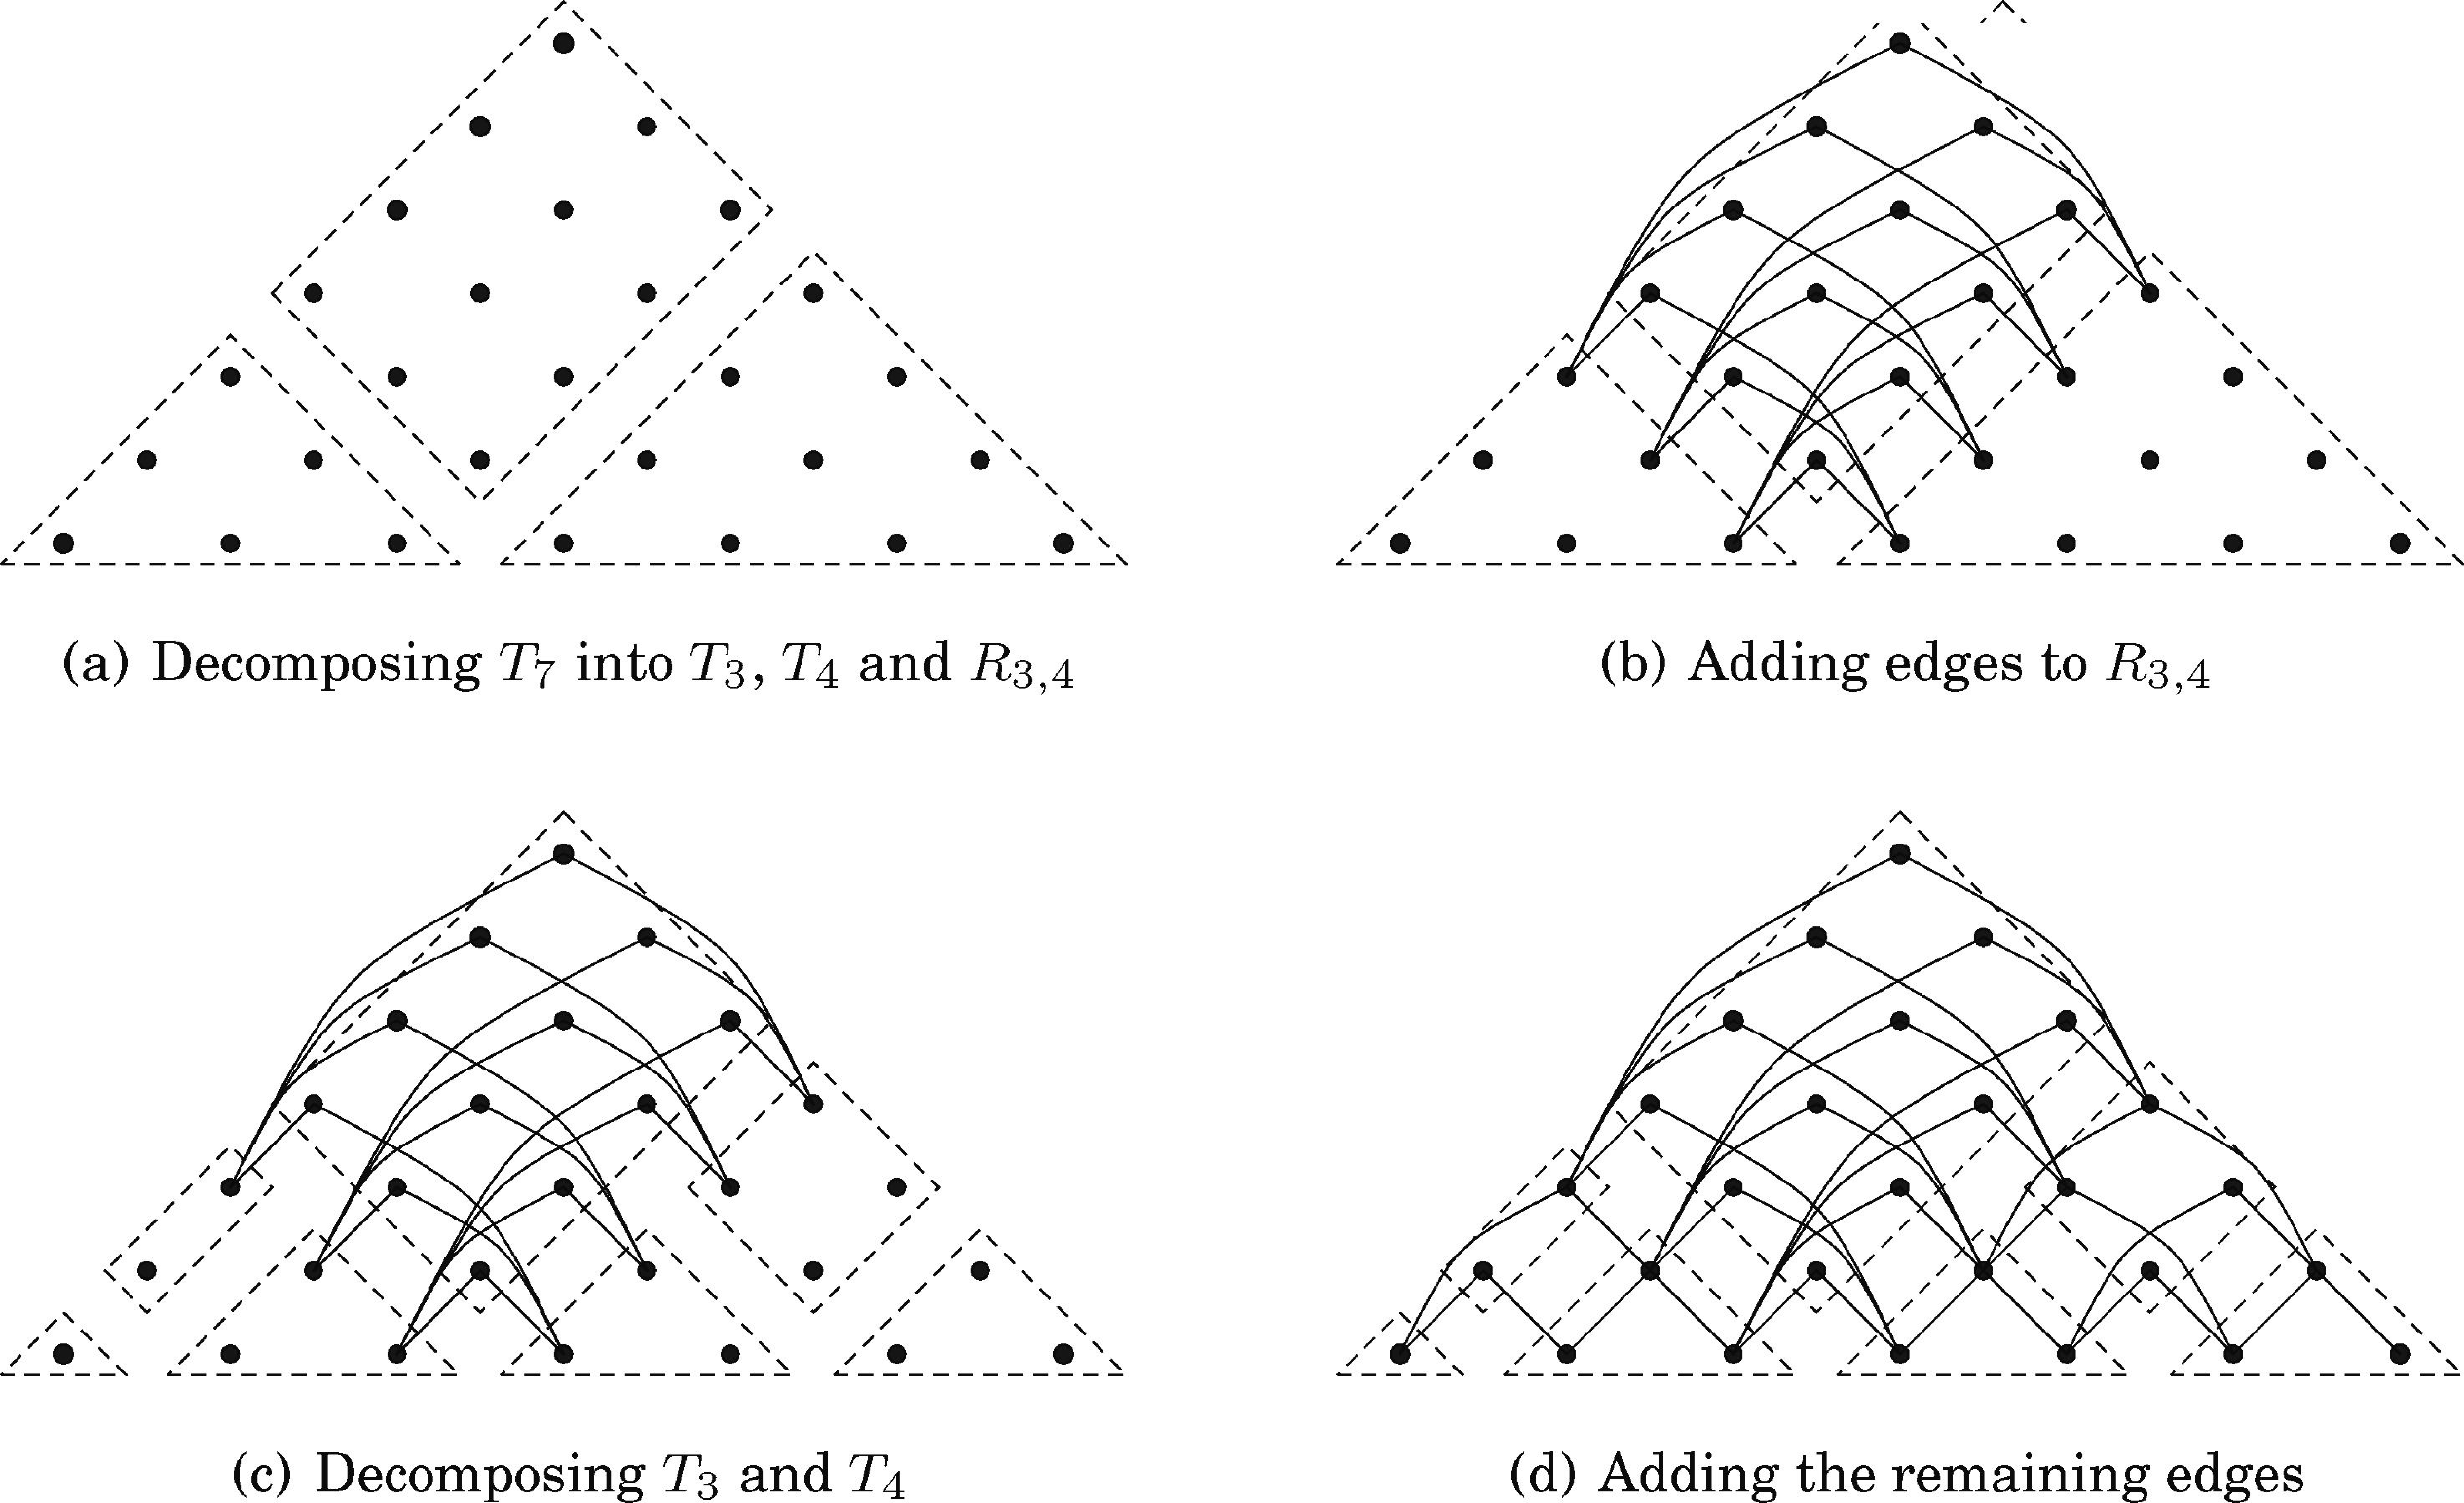
\includegraphics[height=3.0in,width=6in,angle=0]{binarydecompo.pdf}}
\caption{The binary decomposition of $T_{7}$.\cite{mainPaper}}
\label{fig:binarydecomp}
\end{figure}

\subsubsection{Building the Tree}
Crampton[2011]\cite{mainPaper} describes a process of binary decomposition which uses recursive labelling methods to separate the whole tree into nodes. In general the result is a smaller tree with some unnecessary edges being removed meaning that key derivation takes less time and the required storage space for the tree is smaller. The following describes how the process works:
\newline \indent If $T_{m}$ represents the set of intervals where $m$ is the cardinality then ``let $l = \lfloor m/2 \rfloor$ and $r = \lceil m/2 \rceil$. Now $T_{m}$ comprises:
\begin{itemize}
\item A copy of $T_{l}$, containing the minimal elements $[1, 1], \dots , [l,l]$.
\item A copy of $T_{r}$, containing the minimal elements $[l + 1, l + 1], \dots , [m, m]$.
\item A copy of rectangle $R_{l,r}$, containing the remaining nodes in $T_{m}$."
\end{itemize}
The result of this procedure can be seen in Figure ~\ref{fig:binarydecomp}a for $T_{7}$.
\newline The next step is to begin adding edges. An edge is added from every node in $R_{l,r}$ to two other nodes, a single node in $T_{l}$ and a single node in $T_{r}$. ``In particular, for node $[x, y]$ such that $x<l≤y$, we add edges from $[x, y]$ to $[x, l]$ and from $[x, y]$ to $[l + 1, y]$."
\newline This algorithm is then recursively applied to $T_{l}$ and $T_{r}$ until $l, r ≤ 1$. The final result of this process can be seen in Figure ~\ref{fig:binarydecomp}d.
\newline \indent It is clear to see that the information flow policy is still upheld, ie. each node still has access to all other nodes it previously had access to before the binary decomposition however it has not gained access to any new nodes.
\newline \indent Crampton details how this algorithm can be extended to temporal, geo-spatial and general interval access control.

\subsubsection{Assured Delete}
In this system it may be desirable to include reassurances that files which have been restricted from access (which may well happen frequently) are truly unrecoverable. Perlman[2005]\cite{delete} offers measures to achieve this using cryptography in 3 different ways:
\begin{itemize}
\item \textbf{Time-based} - For when files have an expiration date when they are published.
\item \textbf{Individual deletion on-demand} - When files can be deleted individually at any time.
\item \textbf{Custom classes that can be deleted on-demand} - Sets of files (a class) are encrypted with a custom key where the class can be deleted or suspended at any time.
\end{itemize}
While all methods may be applicable in some scenario, most notably the 3rd method has the most parallels with our proposed system. For instance, as all files in a security level must be encrypted with the same key assured delete may be seamlessly applied to all security levels.
\newline \indent This process works mainly by having a trusted authority, one for each class, which controls access to files using a public key and decrypting files (using blind decryption) for the client. In our system it is clear that it would only be suitable for the owner of the filesystem to have access to the public key to encrypt new data and access to the authority would have to be regulated under our own existing access control.

\subsubsection{Programming Languages and Usable Software}
Dropbox has a choice of SDKs which can be used for this project: the options for desktop development are written in Python, Java and Ruby, while there are options for Android and iOS development.
\newline Following is a run down of the different languages and what they offer:
\begin{itemize}
\item Python has a few cryptographic tools available, such as PyCrypto which has a number of hash functions and encryption algorithms ready to use. The low level functions in PyCrypto are written in C for speed.\cite{pyCrypto} Programming in Python is quick and flexible.
\item The main cryptography API available for Java is the Java Cryptography Architecture (JCA) which incorporates two packages, \textit{javax.crypto}, which contains an interface for low level cryptography such as encryption, decryption, and hashing, and \textit{java.security} which contains an interface for key management, certificate management, and signatures. The algorithms to implement the cryptography are included with a Service Provider Interface (SPI), with these there are many symmetric algorithms available such as AES, DES, DESede, Blowfish and IDEA\cite{javaJCA}. An alternative is The Legion of the Bouncy Castle API which incorporates JCA/JCE\cite{bouncyCastle}. Another alternative is The GNU Crypto project which is native on Linux machines and is coded in Java and offers many algorithms including AES, DES, Blowfish. An important point is that "GNU Crypto does not implement any algorithms that are encumbered by patents, and does not rely on any non-free code or documentation."\cite{gnuCrypto}.
\item Ruby offers a module to interface with the OpenSSL cryptography library written in C. The module offers many modern ciphers such as AES.\cite{rubyOpenSSL}
\item It is also possible to create this project in C/C++ using OpenSSL. This can be done by linking the C code to the Dropbox API using Java JNI or creating built-in modules for Python.
\end{itemize}
Keyczar is an API that exists for Java, Python and C++.\cite{keyczar} However it does not appear flexible enough to be used in this case. It is intended for those who have little understanding of cryptography and so it hides too much information to be useful in our case.
\newline As a large part of the evaluation for this project is based around performance I have ignored the possibility of creating the system on a mobile platform where it may not perform to its full potential. As for desktop languages, due to my inexperience with Ruby and wider cryptography support for the other languages available I decided it was not the best language for this project. It also seems unnecessary to take the extra time needed to code the project in C/C++ to risk compatability issues and possible performance hits on linking the languages. While the Dropbox source code is written Python and so may well integrate better with the Python Dropbox API, Java offers a greater range of cryptographic support. The most appealing of the APIs is GNU Crypto as the system will always run on a Linux machine and the lack of unpatented code will prevent the system from becoming tied down if there is a desire to freely distribute it after production.

\section{Project Plan}
Initially the primary goal will be to implement the basic structure of the system which can then be expanded on in many ways. The criteria this structure will need to fulfill are as follows:
\begin{itemize}
\item \textbf{Sharing} - There has to be methods in place which enables a user to share folders or files with other users
\item \textbf{Access Control} - A user has to be able to control which level of access other users have to her files or folders. The implementation should not be dependent on the following:
	\begin{itemize}
	\item \textbf{KAS}
	\item \textbf{Re-encryption policy}
	\item \textbf{Ciphers}
	\item \textbf{Hash functions}
	\end{itemize}
All should be easily changeable.
\item \textbf{Revokation or adjustment} - A user has to be able to remove previously granted permissions or adjust them to a different level.
\item \textbf{Re-encryption} - No particular method needs to be implemented however the system needs to be flexibly accommodating to different methods of re-encryption being 'plug-and-played.'
\item \textbf{Filesystem} - The implementation should not depend on the files being hosted in a certain location.
\newline Coming into this project the initial aim was to implement this system on top of Dropbox's 'public' folder however unfortunately Dropbox has discontinued support for this feature for new users.\cite{dropboxPublicFolder} However Dropbox refers developers to the \textit{/shares} call which enables users to share a file or folder with others.
\newline \indent Once the structure of the system has been created I will begin to create the different implementations of the features discussed.
\end{itemize}

The proposed time scale for this project is as follows:
\begin{itemize}
\item \textbf{Structure} - Two weeks (8th Feb - 22nd Feb). By this time criteria as described should have been fulfilled.
\item \textbf{Algorithms} - Two weeks (22nd Feb - 8th March) By this time the majority of the proposed algorithms to evaluated will have been implemented.
\item \textbf{Assured delete} - One week (8th March - 15th March) - By this time the assured delete method will have been implemented.
\item \textbf{Evaluation} - One week (15th March - 22nd March) - By this time tests will have been carried out for the implemented features.
\item \textbf{Further features/evaluation} - One week (17th May - 24th May) In this time any extra features or evaluations will be implemented or carried out.
\item \textbf{Report} - Three weeks (24th May - 14th June) During this time the report will be written.
\end{itemize}

\section{Evaluation Plan}
To meet the objectives the main criterias to be measured for success are as follows:
\begin{itemize}
\item \textbf{Speed} - To be measured in seconds/milliseconds. Perhaps the most important time interval to measure is,  using a set of test queries, the average time it takes a user to go from probing a file for access to receiving the file. Using a 'correct' set of test queries this metric will give a reading as to how well every feature is performing together. A 'correct' set can be defined as those which activate all features at an appropriate frequency (for instance, a user needs to be revoked permissions to incorporate the re-encryption algorithm into the reading). This measure can be taken with the same features on a number of differently sized trees to show how consistent it remains.
\newline Individual 
\item \textbf{Security} - For each implementation, as a user, attempts can be made to derive information for which they are not permitted to access. There are known attacks for some implementations of hierarchical access control (such as collusion whereby two users with different permission work together to derive forbidden keys) which can be used to test how resistant the implementation is. However known attacks will almost always be applicable meaning that such attacks will only be interesting if the time taken to execute them is drastically reduced. Much of the focus will go to see if there are any security holes, rather than brute force attacks, and how dangerous they may be.
\item \textbf{Ease of use} - Dropbox is famous for its simplicity which will likely make it clear to see if the usability is infringed upon heavily. This could be measured by how many clicks it takes to access a file (vanilla Dropbox takes 1), how many clicks it takes to secure a file, how many clicks it takes to assign permissions and how many clicks it takes to revoke permissions. The time activities take, talked about under '\textit{Speed}' above, will also play into how usable the system is.
\newline \indent While this may be interesting to see and will indicate whether there is any production value for the system, this is not the most important measurement for this project.
\end{itemize}
Some implementations may perform exceptionally well under certain condition and others may perform reasonably well under a small number of conditions and awful in others. To detect such high and low points it is important to thoroughly test each one under as many different conditions as possible.
\newline \indent The main determining factor of how well each implementation performs is the shape and size of the tree. The tree can be manipulated in a number of ways:
\begin{itemize}
\item Increase the number of security levels. This will tend to increase the breadth of the tree.
\item Alter the edges in the tree such that the the number of edges, ($|E|$), becomes high or low, or such that the diameter of the graph, ($d$), becomes high or low. Typically increasing one has the inverse effect on the other. 
\item Assign the user more secret keys. This will have the effect of making tree searches smaller. For instance, going from 1 key to 2 keys potentially halves the size of any one single tree.
\item Force aspects of the graph to conform to maximum, minimum or interval boundaries. This could be applied to the depth, breadth, in-degree and out-degree. A manner to achieve this is to randomly generate a number between 0 and 1 and sum that with the difference between the maximum possible value and the minimum possible value. An example of this can be seen in Table ~\ref{tab:graphGenerator}. This uses truncation to solve the problem of attaining non-integer values after taking the product of the random number and the interval. As can be clearly seen by the in-degree and out-degree examples this raises a problem in which in the interval $[1 \dots 2]$, 1 shall be selected $100/101$\% of the time. This solution will majorly distort the results. A better alternative will be to round the fraction to the nearest integer, however in this example 1 shall be still be selected $51/101$\% of the time compared to 2 being selected $50/101$\% of the time.
\newline \indent Naturally when forcing features of the tree to conform to an interval there are occasions in which one feature will create requirements that another feature will have to abide by to allow the creation of the tree to remain possible. For instance, if the bounds for the out-degree is $1≤x≤1$ where $x$ is the out-degree then the minimum bound for the breadth can be no larger than 1. This is because with a maximum bound of 1 for the out-degree the tree can only be a straight line with breadth 1. Due to this there must be measures in place to ensure that the intervals are controlled to eliminate such conflicts. It can also be noted that even if in the given example the minimum bound obeys the requirements and is no higher than 1, the maximum must be ignored if it is higher than 1 or also be forced to be no higher than 1.
 
\end{itemize}
Upon identifying a particular weakness or flaw in an algorithm, further work can be found by narrowing down the root cause of the problem. If possible, a solution or work around could be devised with the intent to improve upon the algorithm in general or to adapt it to become more applicable to the environment at hand. This new solution could be evaluated independently from the old algorithm.

\begin{center}
\begin{table}
    \begin{tabular}{ | l | l | l | p{5cm} |}
    \hline
    Table feature & Random number & Interval & Result \\ \hline
    Depth & 0.70 & $[2 \dots 7]$ & $0.70 \times (7-2) = 3.5$ \newline \textbf{$3$} \\ \hline
    Breadth & 0.51 & $[3 \dots 9]$ & $0.51 \times (9-3) = 3.06$ \newline \textbf{$3$} \\ \hline
    In-degree & 0.98 & $[1 \dots 2]$ & $0.98 \times (2-1) = 0.98$ \newline \textbf{$1$} \\ \hline
    Out-degree & 0.34 & $[1 \dots 2]$ & $0.34 \times (2-1) = 0.34$ \newline \textbf{$1$} \\ \hline 
    \end{tabular}
    \caption{Generating trees using feature intervals. Takes a random number $x$, where $0≤x≤1$ and fraction results are truncated to reach an integer.} \label{tab:graphGenerator}
    \end{table}
\end{center}

\section{Related work}
Dropbox
Bitbox?
Mega

\section{Implementation}
\subsection{Design}
- Class diagram
- Purpose of each class

\section{Design decisions}
\subsection{Algorithm choices}

\subsection*{Algorithm providers}
There are many different providers of AES algorithms for Java, however there is little literature on the differences between them. This is problematic due to the fact our system is very likely to execute these algorithms very frequently and if the algorithm is inefficient the algorithm may end up becoming an unnecessary bottle neck. The possible ways we can differentiate between the implementations are as follows:
\begin{itemize}
	\item \textbf{Correctness} - The algorithm is implemented correctly.
	\item \textbf{Speed} - The time the implementation takes to execute.
	\item \textbf{Size} - The size of the .jar import needed to use the implementation.
\end{itemize}
Determining the correctness of the implementations is outside of the scope of this report and so it will be assumed all implementations covered here are implemented correctly. The speed and size of the import needed are easy enough to measure and so they are the features we shall be looking at.

\subsubsection*{AES algorithm provider}
\newline The findings for each implementation of AES can be found in Table ~\ref{tab:aesComparison}. As can be seen GNUCrypto is tested with a slightly different algorithm, specifically a different spadding scheme. This is because it does not implement PKCS5 padding (or any in common with the other implementations being tested), only PKCS7. Because of this a fairer comparison would have been to compare each using no padding, which all of them implement, however we have no control over the size of the files the user may encrypt and so the results would have irrelevent to the situation we face. For this reason each implementation used the padding which we would use should it be included in our system. Looking at the table the most striking result is the length of time the GNUCrypto implementation takes. Incorporating the GNUCrpyto implementation into the project is far more complicated than the interface provided by the JCE framework (requiring 15x as much code!) and so that may be an explanation but, in any case, henceforth we shall disregard the GNUCrypto implementation. As for the fastest implementation, there is little between the SunJCE and Bouncy Castle implementations. The real difference is not in speed but in the much more extensive library of ciphers BC provides against not requiring an external jar in the case of SunJCE.

% Comparison of AES implementation features
\begin{center}
\begin{table}
    \begin{tabular}{ | l | l | l | l |}
    \hline
    Implementation & Algorithm & Import Size & Time taken (seconds) \\ \hline
    
    SunJCE & AES/CFB/PKCS5 padding/256bit key & 0 & 14.675065865 \\ \hline
    
    GNUCrypto & AES/CFB/PKCS7 padding/256bit key & 598.0kB & 37.151290762 \\ \hline
    
     Bouncy Castle (via JCA provider) & AES/CFB/PKCS5 padding/256bit key & 2.3MB & 14.700266274 \\ \hline
    
    \end{tabular}
    \caption{Comparisons between different implementations of AES when encrypting a 1.3MB pdf file 1000 times} \label{tab:aesComparison}
    \end{table}
\end{center}

\subsection*{RSA algorithm provider}
GNUCrypto does not provide an implementation of RSA and so it is omitted from the tests.

% Comparison of RSA implementation features
\begin{center}
\begin{table}
    \begin{tabular}{ | l | l | l | l |}
    \hline
    Implementation & Algorithm & Import Size & Time taken (seconds) \\ \hline
    
    SunJCE & RSA/ECB/PKCS1 Padding/2048bit key & 0 & 2.188269064 \\ \hline
    
     Bouncy Castle (via JCA provider) & RSA/ECB/PKCS1 Padding/2048bit key & 2.3MB & 2.356249393 \\ \hline
    
    \end{tabular}
    \caption{Comparisons between different implementations of RSA when encrypting a 256bit AES key 10000 times} \label{tab:rsaComparison}
    \end{table}
\end{center}

\section{Testing}

\section{Evalutation}
\subsection{What I would have done differently}

\section{Conclusion}
\subsection{Future work}

\begin{thebibliography}{10}

\bibitem{appliedCryptoBook}
Bruce Schneier, \emph{``Applied Cryptography: Protocols, Algorithms, and Source Code in C"}, 1995.

\bibitem{newCryptoDirections}
Diffie and Hellman, \emph{``New Directions in Cryptography"},
IEEE Transactions on Information Theory, Vol. IT-22, No.6, 1976.

\bibitem{classicalCryptoBook}
S Vaudenay, \emph{``A Classical Introduction to Cryptography: Applications for Communications Security"}, 2005.

\bibitem{blockCiphers}
A. Menezes, P. van Oorschot and S. Vanstone, \emph{``Handbook of Applied Cryptography"}, Chapter 7, CRC Press, 1996.

\bibitem{accessControlPrinciples}
Sandhu and Samarati, \emph{``Access Control: Princples and Practice"},
IEEE Communications Magazine, September 1994.

\bibitem{dropboxInfo}
\emph{``Dropbox company info"},
Available at: \texttt{https://www.dropbox.com/news/company-info}.

\bibitem{bittorrent}
Fu, Kamara and Kohno, \emph{``Key Regression$\colon$ Enabling Efficient Key Distribution for Secure Distributed Storage"}, 2005.

\bibitem{mainPaper}
Jason Crampton, \emph{``Practical and Efficient Cryptographic Enforcement of Interval-Based
Access Control Policies"}, Royal Holloway, University of London, 2011.

\bibitem{atallahGeo}
Atallah et al, \emph{``Efficient Techniques for Realizing Geo-spatial Access Control"},  Purdue University, 2007.

\bibitem{atallah2005}
Atallah et al, \emph{``Dynamic and Efficient Key Management for Access Hierarchies"}, Purdue University, 2005 (revised 2009).

\bibitem{blanton2007}
Blanton, \emph{``Key Management in Hierarchical Access Control"}, Ph.D. Thesis, Purdue University, 2007.

\bibitem{lazyEncryption}
Jason Crampton, \emph{``Cryptographically-Enforced Hierarchical
Access Control with Multiple Keys"}, Information Security Group, Royal Holloway, University of London, 2009.

\bibitem{largeLeaf}
JW Lo, MS Hwang and CH Liu, \emph{``An Efficient Key Assignment Scheme for Access Control in a Large Leaf Class Hierarchy}, Information Sciences, 2011.

\bibitem{ecc1}
AK Das, NR Paul and L Tripathy, \emph{``Cryptanalysis and Improvement of an Access Control in User Hierarchy Based on Elliptic Curve Cryptosystem"}, Information Sciences, 2012.

\bibitem{ecc2}
YL Lin, CL Hsu, \emph{``Secure key management scheme for dynamic hierarchical access control based on ECC"}, Journal of Systems and Software, 2011.

\bibitem{delete}
Radia Perlman, \emph{``File System Design with Assured Delete"}, Sun Microsystems, 2005.

\bibitem{pyCrypto}
Dwayne C. Litzenberger, \emph{``PyCrypto - The Python Cryptography Toolkit"},
Available at: \texttt{https://www.dlitz.net/software/pycrypto/}.

\bibitem{javaJCA}
\emph{``Java\texttrademark Cryptography Architecture (JCA) Reference Guide"},
Available at: \texttt{http://docs.oracle.com/javase/6/docs/technotes/guides/security/crypto/CryptoSpec.html}.

\bibitem{bouncyCastle}
\emph{``The Legion of the Bouncy Castle"},
Available at: \texttt{http://www.bouncycastle.org/java.html}.

\bibitem{gnuCrypto}
\emph{``The GNU Crypto project"},
Available at: \texttt{https://www.gnu.org/software/gnu-crypto/\#introduction}.

\bibitem{rubyOpenSSL}
\emph{"openssl: Ruby Standard Library Documentation"},
Available at: \texttt{http://www.ruby-doc.org/stdlib-1.9.3/libdoc/openssl/rdoc/index.html}.

\bibitem{keyczar}
\emph{"Keyczar"}, Available at: \texttt{http://www.keyczar.org/}.

\bibitem{dropboxPublicFolder}
Dropbox API Team, \emph{``New sharing model will replace Public folder"},  15th June 2012,
Available at: \texttt{https://www.dropbox.com/developers/blog/19}.

\end{thebibliography}

\end{document}


